
\documentclass[11pt, a4paper, USenglish]{article} % change ``USenglish'' to ``norsk'' if applicable.
%\documentclass[10pt,fleqn,oneside]{article}


\usepackage{kyblab} % Contains all included packages. See kyblab.sty.
\usepackage[a4paper, total={460pt, 690pt},hcentering, bindingoffset=0mm]{geometry}

\addbibresource{riktig.bib} % Makes the bibliography file available to biblatex.

%\setcounter{section}{-3}

\usepackage{amsmath}
\usepackage{graphicx}% http://ctan.org/pkg/graphicx
\usepackage{yhmath}% http://ctan.org/pkg/yhmath
\usepackage{mathdots}% http://ctan.org/pkg/mathdots
\usepackage{MnSymbol}% http://ctan.org/pkg/mnsymbol
\usepackage[toc,page]{appendix}
\usepackage{dirtytalk}
\bibliography{riktig}


\begin{document}

% Titlepage
\title{TTK23 Introduction to Autonomous Robotic Systems for Industry 4.0}
\author{Compendium\\
Hanna Waage Hjelmeland}
\date{March 26, 2021}
\begin{titlepage}
    \maketitle
    \begin{figure}[h]
    \centering
        
\includegraphics[width=\textwidth]{figures/FaultBasics/robot.png}\\   
    \end{figure}

   \thispagestyle{empty}
\end{titlepage}

% Abstract
%\newpage
%\begin{abstract} 
%\addcontentsline{toc}{section}{Abstract} % add this if you want the abstract in the table of contents.
  This document outlines a few important aspects of a lab report. It contains some advice on both content and layout. The \LaTeX{} source for this document is also published, and you can use it as a template of sorts for your own report. You can find an up to date version of the source at \url{https://github.com/ntnu-itk/labreport}. The main file, ``labreport.tex'', defines the structure of the document. The ``preamble.tex'' file is the document preamble, and contains a lot of informative comments. The document is based on work done by Tor Aksel Heirung for TTK4135, and is now under continuous improvement by Andreas L. Fl{\aa}ten and Kristoffer Gryte (happily accepting suggestions and contributions from the community).

When you write your own report, this section (the abstract) should contain a \emph{very} short summary of what the lab is about and what you have done.
\end{abstract}

%\thispagestyle{empty} % Avoid page numbering on the abstract page.
\newpage
% TOC
\newpage
\tableofcontents
\addtocontents{toc}{\protect\thispagestyle{empty}}
\thispagestyle{empty}
% Avoid page numbering on the table of contents.

% Main content
\newpage
\setcounter{page}{1}
\section{MDPS}
\label{sec:mdps}

\subsection{Markov chains}

Markov Chains consists of states and their transition probabilities.

\begin{figure}[h]
    \centering
        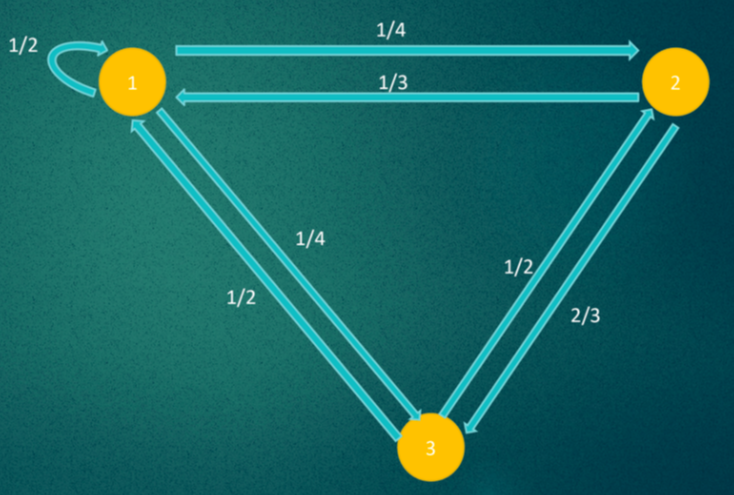
\includegraphics[width=0.8\textwidth]{figures/MDPS/chain.png}\\
        \caption{Markov Chain}
\end{figure}

\subsection{Markov Decision Processes}

A Markov Decision Process is a Markov Chain, in addition to actions and rewards.

\begin{figure}[h]
    \centering
        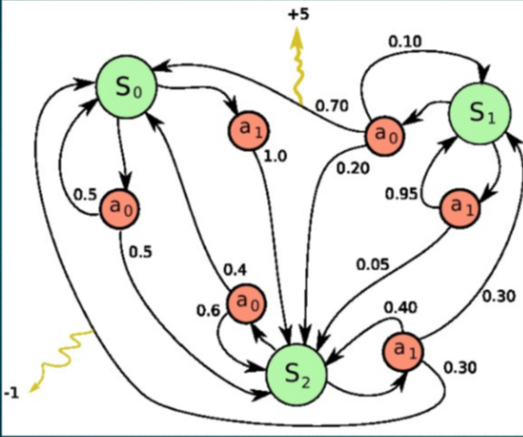
\includegraphics[width=0.5\textwidth]{figures/MDPS/mdp.png}\\
        \caption{MDP Illustrated}
\end{figure}

A markov decision process contains
\begin{itemize}
    \item States
    \item Actions
    \item Transition fucntion
    \item Reward
\end{itemize}



\subsubsection{States}

A MDP state is a unique characterization of all important information in a state of the problem that is modeled. The state space $S$ is the set of environmental states ${s_1, s_2, ..., s_n}$ $\in$ $S$.

\subsubsection{Actions}

The set of actions is the finite set ${a_1, a_2, ..., a_n}$ $\in$ $S$. The action space is restricted by the environmental state and becomes $A(s)$ $\subseteq $ $A$.

\subsubsection{Transition function}

The transition function $T$ is defined as $T: S x A x S -> [0, 1]$. I. e. the transition function takes in a current state, a possible action, and returns the probability of the next state. It is also denoted $T(s, a, s')$.
The transition function adheres to the Markov assumption, that is, the current state s gives enough information to make an optimal decision. Previous states are of no significance.

\subsubsection{Reward function}

The reward function $R: S x A x S -> \mathcal{R}$ takes in a current state, an action from the current state and a possible next state and returns a scalar value. It gives the reward of going from one state to another based on the performed action.


\subsubsection{MDP definition}

A MDP is a tuple $\bigl< S, A, T, R \bigr>$. The transition function $T$ and the reward function $R$ together define the model of the MDP. 

The MDP process becomes a state-action-reward history $(s_0, a_0, r_0), ..., (s_n, a_n, r_n)$.
Episodic tasks is a task of some episodic length, where the goal is to take the agent from a  starting state to a goal state. If a task is episodic, we obtain a state-action-reward history $(s_0, a_0, r_0), ..., (s_{goal}, a_{goal}, r_{goal} $ where the process ends in state $s_{goal}$ and then starts again. 


MDPs can be model based or model free:
\begin{itemize}
    \item \textbf{Model based}: Full transition dynamics and reward distribution is known. This kind of problem can be solved using dynamic programming.
    \item \textbf{Model free}: When there is no model of the environment and the agent has to explore to get familiar with it and optimize its policy.
\end{itemize}


\subsubsection{Policies}

Given an MDP $\bigl< S, A, T, R \bigr>$, the policy $\pi$ is a function $\pi:$ $S$ -> $A$, i. e, it maps the state to an action. 


\subsubsection{Optimality criteria}

\begin{itemize}
    \item With a finite horizon, the agent usually is set to optimize the expected reward over the specified time horizon,  $E \bigl[ \sum_{t=0}^{h} r_t \bigr]$.
    \item With an infinite horizon, the agent is set up to optimize a discounted expected reward, which makes it prioritize rewards in the near future more than distant rewards,
    $E \bigl[ \sum_{t=0}^{\infty} \gamma^t r_t \bigr]$. This also leads to better convergence properties and formal convergence proofs.
    \item One can also optimize for the average reward over a finite horizon,
    $ \lim_{h-> \infty} E \bigl[ \frac{1}{h} \sum_{t=0}^{h} r_t \bigr]$
\end{itemize}

\subsubsection{Value functions and Bellman equations}

The value function is a measure of the value of being in state $s$, and following policy $\pi$ thereafter. The state-value function is a measure of the value of being in state $s$, taking action $a$, and following the policy $\pi$ thereafter. The values returned is the expected sum of rewards. Both functions link optimality criteria to policies, and most learning algorithms for MDPs compute optimal policies by learning value functions.

Greedy policy: Optimal action given the optimal state-value function $V^*$:

\begin{align}
    \pi^*(s) = \text{argmax}_a \sum_{s'} T(s, a, s')(R(s, a, s') + \gamma V^*(s'))
\end{align}

The relation between the state-value function $V^{\pi}(s)$ and the action-value function
$Q^{\pi}(s, a)$ is 

\begin{align}
    V^*(s) = \text{max}_a Q^{\pi}(s, a)
\end{align}

Again, the optimal policy can be described as

\begin{align}
    \pi^*(s) = \text{argmax}_a Q^{*}(s, a)
\end{align}

The state-value function does \textit{not} evaluate the possible actions,
and thus it cannot be optimized in the same manner as the action-value function. In model free approaches where T and R are unknown, Q-functions are learned instead of V-functions. This is due to the fact that we are uncertain about our policy, and it thus makes sense to compare the value of possible actions up against the value of the action chosen by the policy.

\subsubsection{Exploration vs exploitation}

Studies have shown that always choosing the optimal action (greedy policy) has worse convergence properties than when including a probability $\epsilon$ of taking some other action. This makes the agent explore and discover more aspects of the environment than it would have by choosing the optimal action. 






\section{Solving MDPs}
\label{sec:solve}

\subsection{Ways to solve MDPs}

We categorize MDP solving into

\begin{itemize}
    \item Model-based solutions, which solve MDPs that are model based, i. e., full transition dynamics is known. Hereunder we have to methods
    \begin{itemize}
        \item Value iteration
        \item Policy iteration
    \end{itemize}
    \item Model-free solutions, which solve problems where the transition dynamics are unknown.
    \begin{itemize}
        \item Q-learning
        \item SARSA
    \end{itemize}
\end{itemize}

\subsection{Model-based solutions}

\subsubsection{Value iteration}

Value iteration is a method where the value function is estimated first, and then the policy is computed from the value function. The update rule in \Cref{eq:update_V} is used at each step,

\begin{align}
    V_{t+1} &= \max_a \sum_{s'} T(s, a, s')(R(s, a, s') + \gamma V_t(s')) \\
    &= \max_a Q_{t+1}(s, a)
    \label{eq:update_V}
\end{align}
which is guaranteed to converge in the limit towards $V^*$. After it has converged, the policy is computed. We can also observe that the Q-function is computed at the intermediate steps. Because of the max operator, the system becomes unlinear and has to be solved by iteration, as in this method.

\subsubsection{Policy iteration}

The method of policy iteration finds the value function of the policy for the next timestep and compares this to the action-value function at the next timestep. We do

\begin{itemize}
    \item \textbf{Policy evaluation}: Estimate $V^{\pi}$
    \item \textbf{Policy improvement}: Generate alternative policy $\pi' = \text{argmax}_a Q_{t+1}(s, a) \geq \pi$ as a greedy step.
\end{itemize}

If the improvements stop, then the Bellman optimality equation has been satisfied, and $\pi$ is an optimal policy.

In other words, every timestep, we look one step ahead and think "is it wise to follow the policy I have decided on, or is it better to do a different action? If so, the policy is updated with the better action.

In policy iteration there is no max operator and thus the problem becomes linear and we can solve the system of linear equations to find $V^*(s)$.


\textbf{Generalized Policy Iteration (GPI)} is a term used to describe the concept of letting the policy evaluation and policy improvement processes interact. The policy is improved with respect yo the value function, thus being a locally greedy policy, and the value function is driven towards the value function of the policy. This is the case for almost all reinforcement learning algorithms. See \Cref{fig:gpi} for an illustration.

Value iteration and policy iteration thus pushes eachother in order to get a good result.


\begin{figure}[h]
    \centering
        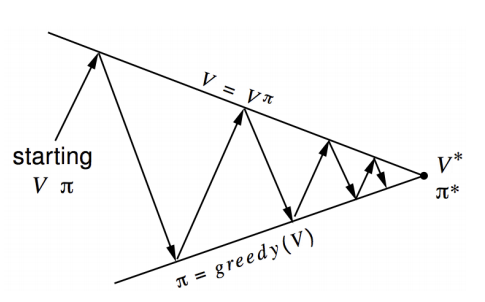
\includegraphics[width=0.8\textwidth]{figures/solving/GPI.PNG}\\
        \caption{The generalized police iteration concept illustrated.}
        \label{fig:gpi}
\end{figure}


\subsubsection{Dynamic programming}

Dynamic programming is often used in model based solvers. Dynamic programming can be used in problems that satisfy the two properties

\begin{itemize}
    \item Optimal substructure: Optimal solution can be decomposed into subproblems
    \item Overlapping subproblems: Subproblems recur many times. Solutions can be cached an reused, as you do in e.g. value iteration, where the temporary value function is stored. 
\end{itemize}

MDPs satisfy both these properties, as the Bellman equations give recursive decomposition, i. e. optimal substructure, and the value function stores and reuses solutions. Again, this is assuming full knowledge of the MDP, as we have in Value Iteration and Policy Iteration.


\textbf{Note}: Sychronous vs asyncronous: updating only some of the states, not the full state space (partiall sweeps).


\subsection{Reinforcement learning and MDPS}
Reinforcement learning is a way to solve problems described as MDPs, when
no prior knowledge about the MDP is presented. This means that the agent has to interact and experiment with the environment in order to gain knowledge about how to optimize its behaviour, guided by the rewards as evaluative feedback.

RL adds to MDPs a focus on approximation and incomplete information, and the need for sampling and exploration. The lack of a model generates the need to sample the MDP and gather statistical knowledge about the unknown model.

\subsection{Model Free solutions}

In model free solutions, we categorize the methods in

\begin{itemize}
    \item \textbf{Indirect/model based RL}: Learning the transition and reward model from interaction with the environment. This can be hard to obtain, and the agent has to learn the characteristics of the environment by exploration.
    \item \textbf{Direct/model free RL}: Estimating value functions or policies directly. 
    \item Mixed forms exist as well.
\end{itemize}

\subsubsection{Temporal credit assignment}

Another aspect of the model free solutions is the temporal credit assignment problem, i. e., when to assign rewards to the agent. It can be difficult to assess the utility of some action, if the real effect of it can only be perceived much later. One possibility is to wait until the end of an episode and punish specific actions along the path. Another possibility is to use similar mechanisms as is value iteration to adjust the estimated value of a state based on the immediate rewars and the estimated (discounted) value of the next state. This is generally called \textbf{temporal difference learning}, and it is a general mechanism underlying model-free methods.


\subsubsection{Online RL}

Online RL is the class of RL algorithms that interact with the environment and update their estimates after each experience. Here the concept of \textbf{exploration vs exploitation} is introduced, which is the concept of choosing a different action than the action that is best according to your current estimate. It is often wise to have a higher exploration rate in the beginning.

\subsubsection{Temporal difference learning}

Temporal difference learning algorithms learn estimates of values based on other estimates, which is called bootstrapping. Each step in the world creates a learning example which can be used to bring some value in accordance to the immediate reward and the estimated value of the next state or state-action pair, and we dont have to wait until the end of a trial to make updates along the path.

TD methods do not require a model of the MDP. Another advantage is that the methods are online and incremental, s. t. they can be easily used in various circumstances.

\subsubsection{TD(0)}

TD(0) Does the job of predicting the value of the next step by estimating the value function with the update rule

\begin{align}
    V_{k+1} &:= V_k(s) + \alpha(r + \gamma V_k(s') - V_k(s)) \\
    \label{eq:td0}
\end{align}


The part $\gamma V_k(s') - V_k(s)$ tells the agent how much it improved by going from state $s$ to $s'$. The backup is performed \textit{after} experiencing the transition from state $s$ to $s'$ based on action $a$ and reward given, $r$.

\subsubsection{Q-learning}

The logic behind Q-learning and TD(0) is the same, except that in Q-learning it is the action-value function that is estimated after an experience. The update rule is a variation of the TD learning scheme,

\begin{align}
    Q_{k+1} &:= Q_k(s, a) + \alpha(r + \gamma \max_{a'} Q_k(s', a') - Q_k(s, a)) \\
    \label{eq:qlearn}
\end{align}

The part $\gamma \max_a Q(s_{t+1}, a)$ returns the maximum possible action value in the state we arrive in, and 
$\gamma \max_a Q(s_{t+1}, a) - Q(s_{t}, a_t)$ thus returns a measure of how much better it is to get to the next state, as in TD(0).

Note that, for both TD(0) and Q-learning, the transition function and reqard function is omitted and a measure of how much better it is to move to a new state is being used instead.

Q-learning is called off-policy because the updated policy is different from the behaviour policy, as it estimates the reward for future actions and appends the value to the new state without actually following a greedy policy. In Q-learning, the agent follows some exploration policy based on Q and an exploration strategy, instead of following the estimated optimal policy directly.

The algorithm is exploration insensitive and will converge to the optimal policy regardless of exploration policy, given that a state-action pair can be visited infinite times and $\alpha$ is decreased properly.

\subsubsection{SARSA}

The SARSA method is a lot like Q-learning, but without the maximum in the update step.

\begin{align}
    Q_{k+1} &:= Q_k(s, a) + \alpha(r + \gamma Q_k(s', a') - Q_k(s, a)) \\
    \label{eq:qlearn}
\end{align}

Instead of the max function to find the best estimated action, the action is chosen directly from an $\epsilon$-greedy policy. Hence, its an \textbf{on-policy} algorithm.

\textbf{Difference between Q-learning and SARSA}:
\begin{itemize}
    \item In both cases the action chosen is chosen from an $\epsilon$-greedy policy.
    \item They differ in the way Q is updated after the action, as SARSA still uses the $\epsilon$-greedy policy here, while Q-learning uses a greedy policy with the max-operator. 
    \item Q-learning is more aggressive and will take shortest paths because they are optimal, while SARSA will take longer, safer routes to avoid unexpected negative rewards. Thus, if mistakes are costly, SARSA should be chosen over Q-learning.
\end{itemize}

\begin{figure}[h]
    \centering
        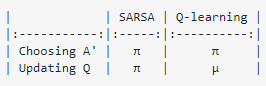
\includegraphics[width=0.5\textwidth]{figures/solving/sarsa_q.PNG}\\
        \caption{Difference between Q-learning and SARSA. $\pi$ is the $\epsilon$-greedy policy, while $\mu$ is a greedy policy.}
\end{figure}

\subsubsection{Monte Carlo}

Different class of methods that solves these types of problems in a different manner (det var alt han sa i forelesning).


\subsection{Policy Gradient Methods}

\subsubsection{From policy iteration to policy search}

Weakness of policy iteration: policies are learned via value functions. Improving the estimate of the value function does not \textbf{necessarily} contribute to improving the policy. Also, a small change in value functions can cause a big difference in policy, which can be very problematic in physical systems s. a. robots. Also, policy improvement (maxiimizing Q) is computationally expensive when the action space A is continous.

\textbf{Policy search overcome these weaknesses}. In policy search, we directly find the policy that maximizes the expected return:

\begin{align}
    \pi^* = \max_{\pi} \mathbf{E}[R]
\end{align}

Policy search addresses the issue of finding a good policy function in a vast function space. 

\textbf{Challenges in policy search}: High varience, instabilities, etc.

\subsubsection{Parameterized policy}

We consider methods that learn a parameterized policy without consulting a value function. A value function may still be used to learn the policy parameter, but is not required for action selection. The policy parameter vector is denoted 

\begin{align}
    \theta \in \mathbf{R}^{d'}
\end{align}

The probability of action $a$ at time $t$ given environment state $s_t$ with parameter vector $\theta$ is given by

\begin{align}
    \pi(a|s, \theta) = P\{A_t = a| S_t = s, \theta_t = \theta\}
\end{align}

\subsubsection{Objective and optimization}

In order to maximize performance, policy gradient methods do gradient ascent steps:

\begin{align}
    \theta_{t+1} = \theta_t + \alpha \widehat{\nabla J(\theta_k)}
\end{align}

where $\widehat{\nabla J(\theta_k)}$ is a stochastic estimate whose expectation approximates the gradient of the performance measure w. r. t. $\theta$. \textbf{All methods that follow this schema are called policy gradient methods, whether or not they learn an approximate value function}. Methods that learn both policy and value functions are called \textbf{actor-critic methods}.

The policy can be parameterized by any means, e.g. deep neural nets, as long as $\pi(a|s, \theta)$ is differentiable w.r.t $\theta$. If the action space is discrete and not too large, we can form parameterized numerical preferences $h(s, a, \theta)$ for each state-action pair. The actions with the highest preferences in each state are then given the highest probabilites, e. g. by a softmax-function:

\begin{align}
    \pi(a|s, \theta) = \frac{e^{h(s, a, \theta}}{\sum_b e^{h(s, b, \theta}}
\end{align}

\subsubsection{The policy gradient theorem}

How much does the expected return increase, for each small change in our policy? 

The policy gradient theorem tells us how we can estimate the performance change with respect to the policy parameter, when the gradient depends on the unknown effect of policy changes on the state distribution. It also gives convergence guarantees that are stronger than for action-value-methods such as $\epsilon$-greedy action selection. 

\begin{align}
    \nabla J(\theta) \propto \sum_s \mu(s) \sum_a \nabla \pi(a|s)Q(s, a)
\end{align}

where $\mu(s)$ is the on-policy state distribution under $\pi$, mgiving a weight that symbolizes how often a state occur under the target policy $\pi$.

\subsubsection{REINFORCE: Monte-Carlo Policy Gradient}

\begin{figure}[h]
    \centering
        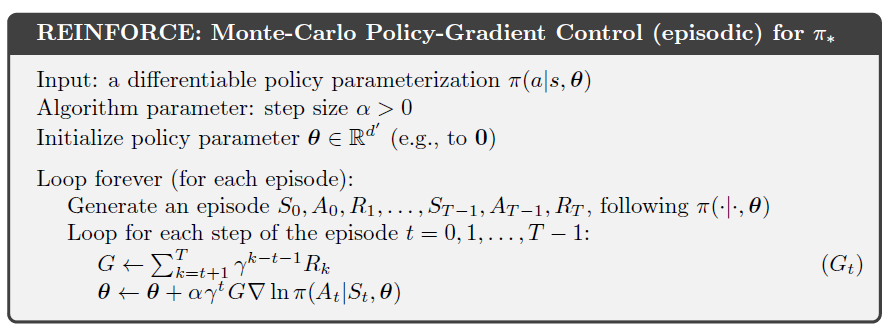
\includegraphics[width=0.9\textwidth]{figures/solving/policy_gradient/reinforce.PNG}\\
        \caption{The policy-gradient method REINFORCE. G denotes the expected return.}
        \label{fig:gpi}
\end{figure}

\textbf{Drawbacks of the reinforce algorithm}:
\begin{itemize}
    \item Full episodes are required before starting to train. Might be OK for short experiments, but for others it is a big problem.
    \item The high gradient varience.
    \item Exploration: It is possible to converge to a locally-optimal policy and to stop exploring. In DQN this is solved via $\epsilon$-greedy action selection, and there are ways to cope with this in policy-gradient methods as well.
\end{itemize}


\section{Deep Reinforcement Learning}
\label{sec:drl}


\subsection{Deep Neural Networks}

\subsubsection{History of NNs}

\begin{itemize}
    \item[\textbf{1940}]: Electronic brain
    \item[\textbf{1957}]: The perceptron 
    \item[\textbf{1960-1970}]: Golden Age, ADALINE: first single layer neural network. 
    \item[\textbf{1970-1986}]: The XOR problem spawns the Dark Age (AI Winter). 
    \item[\textbf{1986}]: Multi-layered perceptron + backpropagation 
    \item[\textbf{1995}]: Support Vecor Machines 
    \item[\textbf{2006}]: Deep Neural Networks
\end{itemize}

\subsubsection{Notes}

\begin{itemize}
    \item Changing parameters according to the error measurement will cause the system to jump around to much and be very effected by noise. That is why the learning rate is introduced.
    \item Observations suggest neurons do not react readily, but instead suppress the input until it has grown large enough to trigger the output. This notion of a threshold is implemented by the activation function.
\end{itemize}


\subsection{The large state space problem}

Both value iteration and Q-learning does a loop over all states. This is challenging when the state space is very large. E. g. the Atari game has $128*{33600}$ possible frame configurations -> billions of billions of years to enumerate all possible states -> curse of dimensionality, recognized by Bellman.

Instead, we want to use a nonlinear representation that maps both state and action onto a value, as a regression problem. This is a job for neural networks.

\subsubsection{Deep Q-learning (DQN)}

The model in DQN is a convolutional neural netwok, trained with a variant of Q-learning, whose input is raw pixels and whose output is a value function estimating future rewards. \textbf{The network estimates the action-value function Q}.

The estimation of Q(s, a) by parameter vector $\theta$ is given as $Q(s', a'; \theta)$. 

\begin{align}
    Q(s, a) &\longleftarrow Q(s, a) + \alpha(r + \gamma \max_a' Q(s', a') - Q(s, a)) \\
    \theta  &\longleftarrow \theta + \alpha(r + \gamma \max_a' Q(s', a'; \theta) - Q(s, a; \theta))\nabla_{\theta}Q(s', a'; \theta)
\end{align}

\subsection{The challenges of Deep Reinforcement Learning}

\begin{itemize}
    \item In RL, both the input and the target change constantly during the training process, which makes training unstable. Hard to learn a mapping that is constantly changing.
    \item In supervised learning, the label stays the same for a given input, and this makes every batch have the same data distribution. Samples are also independent of each other in the same batch. 
    \item Thus, a problem for RL algorithms is that the data is \textbf{highly correlated} and there are \textbf{non-stationary probability distributions}.
\end{itemize}

\textbf{Solutions to challenges}

\begin{itemize}
    \item Experience replay: Randomly sampling previous transitions and replay this. This smoothens the training distribution over many past behaviours.
    \item Make the system obtain a separate target network with weight-vector $\theta^-$ to create a temporal gap between the target action-value function and the action-value function that updates continually.
\end{itemize}

\begin{figure}[h]
    \centering
        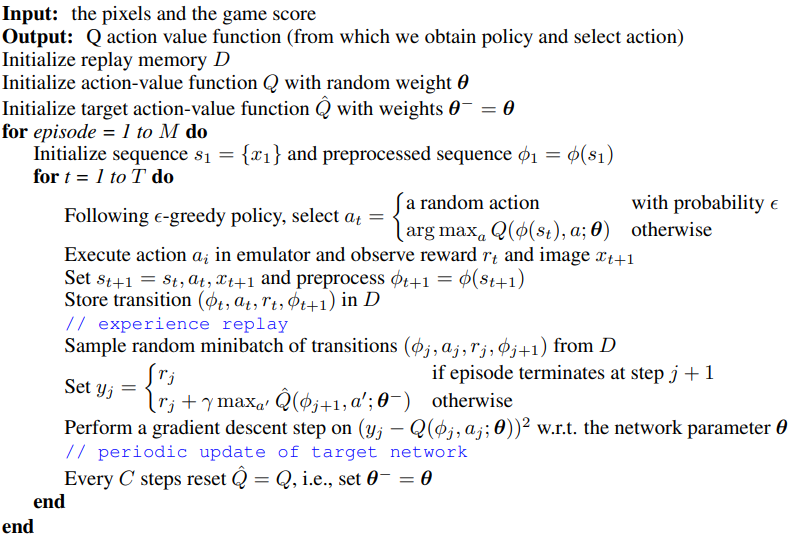
\includegraphics[width=\textwidth]{figures/DRL/dqn.PNG}\\
        \caption{Deep Q-learning pseudocode.}
\end{figure}

The gradient descent step is performed based on the least squares measure of the difference of the reward we obtained and the discounted target action-value function from that step, and the action-value function defined by the network parameter $\theta$.
\section{Explainable Artificial Intelligence (XAI)}
\label{sec:xai}


\subsection{Legal requirements}

\textbf{GDPR}: "An explanation of the decision reached after algorithmic assesment"

\begin{itemize}
    \item Curse of dimensionality: Impossible to collect enough data to represent the problem.
    \item XAI is a young research field. Explantion is not well-defined.
    \item \textbf{Shapley decomposition}: Best way to "poke the box". Characteristic function values: The value of the combinations of the parts.
\end{itemize}





% \input simply inserts the contents of the file, while \include forces a \newpage.
% See \input vs. \include: http://tex.stackexchange.com/questions/246/when-should-i-use-input-vs-include

% References
\newpage
%\addcontentsline{toc}{section}{References}
\printbibliography
\label{sec:bibliography}

\end{document}
